% ---------------------------------------------------------------------------
\section{Results on Development Flows}\label{sec:dev-results}
\noindent
{\bfseries RQ1 (quality).} Does the teacher improve detection quality over students trained without it, and does the answer depend on which teacher signal is distilled? {\bfseries RQ2 (fidelity).} Does score distillation transfer the teacher's scoring behavior? {\bfseries RQ3 (attribution).} Is any failure attributable to the score interface itself, rather than to context asymmetry, teacher capacity, or the training constraint?
% ---------------------------------------------------------------------------

This section reports the exploration stage on the 20 development flows:
the preregistered main grid (arms A/C $\times$ two backbones $\times$ 5
seeds), the auxiliary arms at 3 seeds (B1, B2, AB, LINEAR), and the fixed
references (frozen teacher T0, PCA). All 820 training runs completed without
failure; per-flow seed dispersion is included in the artifact package.

\subsection{The Full Picture}\label{sec:dev-picture}
Table~\ref{tab:dev} reports VUS-PR for eleven arms, the teacher, and PCA
across all development flows. Three observations structure everything that
follows. First, \emph{no method dominates}: the best per-flow arm changes
across flows, and the fixed-configuration PCA baseline (the preregistered strong
classical reference) attains the highest macro mean (0.286) and median
(0.149) while failing catastrophically on specific flow types. The gas-heating loop
is the sharpest single demonstration of the interface effect in our
data. On this one flow, the teacher, every score-distilled student
(0.008--0.013, including the AB hybrids), and PCA (0.007) all collapse,
while the two
forecast-trained students reach 0.38--0.44. Second, \emph{eight of the ten neural student arms exceed the
teacher's macro mean} (the exceptions are the two TCN variants trained
on the teacher's weakest signal, A-TCN 0.137 and AB-TCN 0.130 vs.0.165); the best per-flow student beats the teacher on 16 of 20 flows
(2 losses, 2 ties). The teacher is a weak spot on its own grid, echoing the
condition-dependence reported by zero-shot audits. Third, the \emph{interface} of the distillation signal
matters more than the presence of a teacher. Self-supervised and
forecast-distilled students (B1/B2/LINEAR, 0.217--0.253 macro) dominate
score- and ranking-distilled students (A/C, 0.137--0.180).

% AUTO-GENERATED from results/m5*/ — do not edit numbers by hand
\begin{sidewaystable}
\centering
\caption{Development-set VUS-PR (mean over seeds) for eleven arms, the frozen teacher (T0), and the preregistered PCA baseline across the 20 dev flows. Best per flow in bold.}
\label{tab:dev}
\scriptsize
\setlength{\tabcolsep}{2.4pt}
\begin{tabular}{lccccccccccccc}
\toprule
Flow & C-PM & C-TCN & A-PM & A-TCN & B1-TCN & B1-PM & B2-TCN & B2-PM & AB-PM & AB-TCN & LINEAR & T0 & PCA \\
\midrule
D10\_GHL\_id2 & 0.008 & 0.008 & 0.011 & 0.012 & 0.438 & 0.435 & \textbf{0.438} & 0.435 & 0.013 & 0.013 & 0.383 & 0.009 & 0.007 \\
D11\_SVDB\_id2 & 0.061 & 0.058 & 0.060 & 0.059 & 0.081 & \textbf{0.092} & 0.081 & 0.091 & 0.061 & 0.059 & 0.091 & 0.067 & 0.069 \\
D12\_EMG & 0.119 & 0.116 & 0.117 & \textbf{0.119} & 0.118 & 0.119 & 0.118 & 0.119 & 0.118 & 0.116 & 0.118 & \textbf{0.119} & 0.071 \\
D13\_JD1\_svc0 & 0.014 & 0.019 & 0.015 & 0.016 & 0.009 & 0.008 & 0.009 & 0.009 & 0.015 & 0.016 & 0.008 & 0.073 & \textbf{0.695} \\
D14\_NAB\_cpu24ae8d & 0.140 & 0.226 & 0.202 & 0.196 & 0.183 & 0.236 & 0.178 & 0.234 & 0.201 & 0.202 & \textbf{0.305} & 0.222 & 0.136 \\
D15\_NAB\_cpu53ea38 & 0.304 & 0.292 & 0.304 & 0.298 & 0.294 & 0.291 & 0.292 & 0.293 & 0.288 & 0.297 & 0.305 & 0.281 & \textbf{0.330} \\
D16\_NAB\_occ6005 & 0.560 & 0.108 & 0.550 & 0.018 & \textbf{1.000} & 0.483 & \textbf{1.000} & \textbf{1.000} & 0.516 & 0.017 & \textbf{1.000} & 0.200 & 0.036 \\
D17\_NAB\_machtemp & 0.297 & 0.397 & 0.350 & 0.427 & 0.457 & 0.260 & \textbf{0.459} & 0.286 & 0.344 & 0.396 & 0.334 & 0.328 & 0.284 \\
D18\_Exathlon\_id1 & 0.481 & 0.550 & 0.273 & 0.117 & 0.915 & 0.925 & 0.933 & 0.922 & 0.656 & 0.100 & 0.947 & 0.561 & \textbf{0.999} \\
D19\_OPP\_id3 & 0.202 & 0.257 & 0.180 & 0.214 & 0.160 & 0.160 & 0.160 & 0.160 & 0.176 & 0.226 & 0.158 & 0.255 & \textbf{0.439} \\
D1\_SWaT\_id1 & 0.542 & 0.524 & 0.424 & 0.396 & 0.545 & \textbf{0.568} & 0.540 & 0.567 & 0.384 & 0.350 & 0.503 & 0.331 & 0.446 \\
D20\_GECCO\_id1 & 0.015 & 0.014 & 0.011 & 0.014 & 0.014 & 0.014 & 0.014 & 0.014 & 0.013 & 0.014 & 0.013 & 0.014 & \textbf{0.403} \\
D2\_HAI & 0.013 & \textbf{0.018} & 0.014 & 0.014 & 0.016 & 0.013 & 0.015 & 0.015 & 0.014 & 0.013 & 0.012 & 0.015 & 0.013 \\
D3\_SMD\_id4 & 0.055 & 0.069 & 0.068 & 0.050 & 0.044 & 0.028 & 0.044 & 0.028 & \textbf{0.070} & 0.048 & 0.032 & 0.069 & 0.040 \\
D4\_SMD\_id20 & 0.030 & 0.061 & 0.161 & 0.099 & 0.078 & 0.023 & 0.071 & 0.023 & 0.046 & 0.084 & 0.042 & 0.030 & \textbf{0.885} \\
D5\_PSM & 0.372 & 0.416 & 0.419 & 0.392 & 0.382 & 0.381 & 0.352 & 0.383 & 0.393 & 0.350 & 0.380 & 0.388 & \textbf{0.501} \\
D6\_MSL\_id10 & 0.085 & 0.088 & 0.090 & 0.098 & 0.105 & 0.100 & 0.105 & 0.100 & 0.089 & 0.096 & \textbf{0.107} & 0.101 & 0.080 \\
D7\_MSL\_id5 & \textbf{0.207} & 0.109 & 0.155 & 0.106 & 0.129 & 0.107 & 0.126 & 0.112 & 0.151 & 0.110 & 0.126 & 0.129 & 0.162 \\
D8\_SMAP\_id4 & 0.059 & 0.060 & 0.059 & 0.059 & 0.058 & 0.060 & 0.059 & 0.060 & 0.059 & 0.060 & 0.058 & 0.065 & \textbf{0.080} \\
D9\_SMAP\_id13 & \textbf{0.037} & \textbf{0.037} & \textbf{0.037} & \textbf{0.037} & \textbf{0.037} & \textbf{0.037} & \textbf{0.037} & \textbf{0.037} & \textbf{0.037} & \textbf{0.037} & \textbf{0.037} & \textbf{0.037} & \textbf{0.037} \\
\midrule
Macro mean & 0.180 & 0.171 & 0.175 & 0.137 & 0.253 & 0.217 & 0.251 & 0.244 & 0.182 & 0.130 & 0.248 & 0.165 & 0.286 \\
Median & 0.102 & 0.098 & 0.136 & 0.099 & 0.123 & 0.113 & 0.122 & 0.115 & 0.104 & 0.090 & 0.122 & 0.110 & 0.149 \\
\bottomrule
\end{tabular}
\end{sidewaystable}

\subsection{Fidelity--Quality Decoupling}\label{sec:dev-fidelity}
If distillation transferred the teacher's scoring behavior faithfully,
the student's scores would correlate strongly with the teacher's. The data refute this. Across the 389 main-grid
runs with finite fidelity (of 400; the remainder yield constant score
vectors), the median teacher--student Spearman $\rho$ is 0.184; only 22\% of
runs exceed $\rho>0.5$, while 53\% fall below 0.2 (Figure~\ref{fig:fidelity}). The decoupling is
flow-structured rather than noise. On the three flows where the median
$\rho$ is highest (SVDB $\rho{\approx}0.84$, MSL-5 $\rho{\approx}0.70$,
J-D $\rho{\approx}0.61$), students track the teacher closely and inherit
its level of performance. On the flows where students improve most over
the teacher (e.g., SWaT: student 0.54 vs.\ teacher 0.33 with
$\rho{\approx}-0.10$; NAB-occupancy: 0.56 vs.\ 0.20; machine-temperature:
0.43 vs.\ 0.33), the student is \emph{not} imitating the teacher at all.
The mechanism is consistent with these observations, which we state as a
hypothesis rather than a proof. Under the normal-only training constraint,
the teacher's scores act as a noisy, weakly informative regression target,
and the measured gains come from the student's inductive bias filtering
this target, a regularization effect, rather than from behavioral
transfer.
The preregistered fidelity companions agree. Across the same 389 runs,
top-5\% score-set overlap averages 0.242 (median 0.151; chance
is 0.05) and pairwise agreement on non-tied teacher pairs averages
0.594, above chance but far from imitation. Anomaly-tail fidelity tells the same story from the deployment
angle and is reported per flow in the artifact package.

\subsection{The Interface Ladder}\label{sec:dev-ladder}
The preregistered three-level comparison asks \emph{which
distillation objective is strongest}. Ranking the objectives by their
information content about the anomaly (ground-truth-free self-supervision B1,
the teacher's \emph{forecast} B2, and the teacher's \emph{score} A/C)
produces a consistent macro separation
(B1/B2/LINEAR $\approx 0.22$--$0.25$ vs.\ A/C $\approx 0.14$--$0.18$),
though within the upper family the B1-vs-B2 ordering swaps with the
backbone (B2-TCN 0.251 edges out B1-PM 0.217's family range; on the
confirmation set the same comparison reverses, Section~\ref{sec:confirm-comparisons}).
Score-level distillation, the interface this paper set out to test, is the
weakest of the three; the pairwise per-flow record confirms it is not a
macro artifact (B1-TCN beats C-PM on 11 of 20 flows). Notably, a linear
predictor with residual scoring (0.248 macro) comes within 0.003 of the
strongest distilled neural student on development (B2-TCN 0.251)
and is the strongest student arm on held-out sources (0.323). The AB arm, which couples score distillation with
forecast alignment, recovers part of the gap over pure score distillation
(AB-PM 0.182 vs.\ A-PM 0.175 at macro) but remains far below
forecast-only training (B2-PM 0.244), indicating that the alignment
benefit comes from the forecast target itself rather than from the
combination.
An interface ablation (revision R7, exploratory) addresses the main
confound directly. Retraining A-PM and B1-PM at the teacher's own
context length ($L{=}512$ instead of 128) on five representative flows
leaves the ladder intact. The B1$-$A difference is $+0.148$ at
$L{=}512$ vs.\ $+0.144$ at $L{=}128$ (per-flow direction agrees on 4 of
5; the disagreement is the occupancy flow). On these five flows, the
context-length asymmetry between teacher and student does not support
an explanation of the interface gap.

A teacher-on-anomaly control (revision R8, exploratory) tests whether
the normal-only training signal, rather than the interface itself, is
the binding constraint. Synthetic anomalies (1\% spikes, 1\% 100-point
level shifts, $k\in\{3,5,8\}\sigma$) are injected into the training
segments of five representative flows; the injection parameters are chosen
independently of the students' window-residual mechanism (spike and
level-shift morphologies, not residual-shaped anomalies), so no arm is
favored by construction; the teacher scores the augmented
segments (its score discriminates injected from normal points on three
of five flows, ratios 1.2--2.8$\times$), and A-PM and B1-PM are
retrained on the augmented streams. The result is sharply bimodal
(Figure~\ref{fig:r8bimodal}).
Where the teacher discriminates, score distillation with anomaly
exposure improves dramatically (Exathlon: $0.27\to0.86$); where it does
not (occupancy: teacher ratio $<1$), augmented distillation degrades
equally dramatically ($0.55\to0.08$). The self-supervised control is
robust to the same augmentation (mean change $+0.001$, per-flow range
$-0.002$ to $+0.008$ across the five
flows). The score interface, then, is not categorically unable to
transfer detection behavior. It inherits the teacher's
condition-dependent inconsistency. Deploying it is a bet on the teacher
responding informatively to the anomalies at hand, and verifying the
bet requires running the teacher on representative data, an offline
cost that is amortized across deployments but still non-trivial
compared to fully self-supervised training.

\begin{figure}[t]
\centering
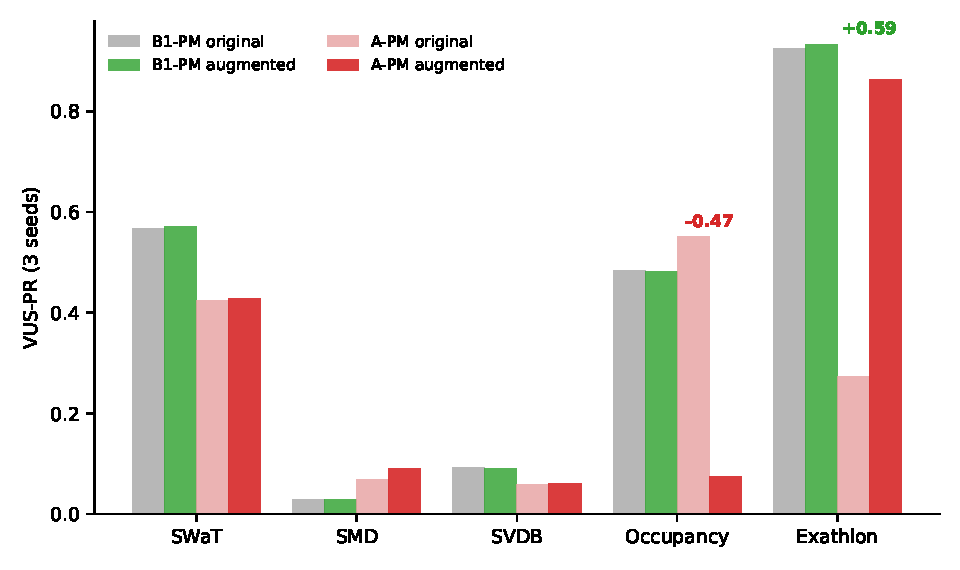
\includegraphics[width=0.8\textwidth]{figures/fig_r8_bimodal.pdf}
\caption{Teacher-on-anomaly control (R8, exploratory): VUS-PR (mean of
3 seeds) on five development flows, four bars per flow. Gray/green:
B1-PM trained on original vs.\ anomaly-augmented segments; light
red/red: A-PM original vs.\ augmented. Bold annotations give the
within-arm augmented-minus-original difference for A-PM (the same
quantity quoted in the text). The outcome is bimodal. Where the
teacher's scores discriminate the injected anomalies, augmented score
distillation improves sharply (Exathlon: $0.27\to0.86$); where they do
not (Occupancy, teacher ratio ${<}1$), it degrades sharply
($0.55\to0.08$). B1-PM is robust to the same augmentation on all five
flows.}
\label{fig:r8bimodal}
\end{figure}

\subsection{Conditional Analysis: When Is Each Arm Worth It?}\label{sec:dev-conditional}
Although PCA tops the macro table, its wins concentrate on flows with
abrupt level/regime anomalies (e.g., Exathlon, SMD-20, J-D), where
reconstruction error separates regimes almost perfectly; on
temporally structured or persistence-type anomalies its failures are
severe (gas-heating loop 0.007; SWaT 0.446 vs.\ student 0.542).
Ranking- and score-distilled students occupy a complementary niche. Their strongest
flows (SWaT 0.542; NAB-occupancy 0.561; machine-temperature 0.428 under
A-TCN) are precisely those where the teacher is weak and where temporal
persistence matters. Per-flow win counts summarize the picture. The
best-per-flow student beats PCA on 11 of 20 flows (loses 8, ties 1) and
beats the teacher on 16 (loses 2, ties 2). Section~\ref{sec:confirm}
tests whether this conditional structure replicates on held-out sources;
Section~\ref{sec:discussion} condenses it into a practitioner selection
table.

\subsection{Negative and Boundary Results}\label{sec:dev-negative}
Reported in full per the preregistration: (i) score-level distillation
does not transfer teacher behavior faithfully (median $\rho$ 0.184) and
does not beat self-supervision; (ii) the ranking objective (C) beats the
score objective (A) at macro on both backbones, but the advantage is
driven by two flows and flips at the median (A-PM 0.136 vs.\ C-PM 0.102),
so we do not claim it as systematic; (iii) one development-set flow
(SMAP-13) is undetectable by \emph{every} method including the teacher
(single anomaly window in the context-undefined region); (iv) the AB arm's
forecast-alignment term does not close the gap to forecast-only training.
